% Provenance (never printed): cycle 4 SVT, "La planete Terre, l'environnement
% et l'action humaine": natural risks, hazard and vulnerability, prevention
% and protection; see sources/book1/PROVENANCE.md. Book 1, grade 9, chapter 2.
% Vocabulary guard: owns risk, vulnerability, prevention, hazard map.
% Natural hazard and natural disaster, the warning colours and the safety
% rules are g5's (natural-hazards); the warning signs of an eruption and the
% Pinatubo story are g7's (volcanoes); seismometer, tsunami and "scientists
% cannot predict earthquakes" are g7's (earthquakes); flood and floodplain
% are g5's (water-shapes-the-land); weather forecast is g8's. Lahars are
% called mudflows (as in g7). "Normal fault" is Book 2's: here "a fault".
\chapter{Living with Natural Risks}\label{ch:g9:natural-risks}

Late in the evening of 13~November 1985, most of the people of Armero, a
town of Colombia, were in bed. A \omterm{def:g5:natural-hazards:storm}{storm} hid the snow-capped \omterm{def:g4:volcanoes-earthquakes-first-look:volcano}{volcano} Nevado
del Ruiz, \qty{45}{km} away, and nobody in the town saw it erupt. The hot
\omterm{def:g3:stones-pebbles-sand:rock}{rocks} melted part of its ice, and the water, mixed with ash and \omterm{def:g3:stones-pebbles-sand:rock}{rock},
rushed down the \omterm{def:g1:landscapes-around-us:landform}{valleys} as mudflows. About two hours later, the mudflows
poured out of the \omterm{def:g1:landscapes-around-us:landform}{valley} of the \omterm{def:g1:landscapes-around-us:water}{river} Lagunillas, straight into the town:
some \num{23000} people, most of the town, were killed. Two hours was time
enough to walk to higher ground. The people of Armero were not told.
% ledger: usgs:armero

\begin{omfigure}
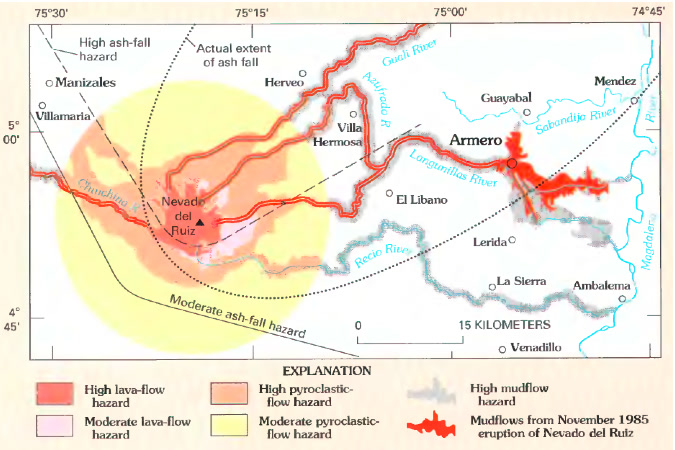
\includegraphics[width=0.86\linewidth]{images/book1/g9-ruiz-hazard-map.jpg}

{\small The \omterm{def:g9:natural-risks:hazard-map}{hazard map} of Nevado del Ruiz. A first version, drawn by
Colombian geologists, circulated one month before the \omterm{def:g4:volcanoes-earthquakes-first-look:eruption}{eruption} and
already showed the danger of mudflows in the \omterm{def:g1:landscapes-around-us:landform}{valley} of Armero. This
version, redrawn after the disaster, adds in bright red the mudflows that
really came in November 1985 (the shaded circle around the \omterm{def:g4:volcanoes-earthquakes-first-look:volcano}{volcano} has a
radius of about \qty{20}{km}). From R.~Wright and T.~Pierson, USGS
Circular 1073, 1992 (public domain, via Wikimedia Commons).}
% ledger: usgs:ruiz-map, commons:ruiz-map
\label{fig:g9:natural-risks:ruiz}
\end{omfigure}

Six years later, at Mount Pinatubo in the Philippines, the \omterm{def:g4:volcanoes-earthquakes-first-look:volcano}{volcano} was
watched, the warning came in time and the people left
(\cref{ch:g7:volcanoes}). Both were explosive \omterm{def:g4:volcanoes-earthquakes-first-look:volcano}{volcanoes}, with people
living in the path of their mudflows. What differed was what people
knew, and what they did with it. This chapter
is about that difference.
% ledger: usgs:armero (Pinatubo 1991 averted a disaster like Armero), usgs:pinatubo-1991

\begin{recall}
A \emph{\omterm{def:g5:natural-hazards:hazard}{natural hazard}} is a natural event that can harm people; it
becomes a \emph{\omterm{def:g5:natural-hazards:disaster}{natural disaster}} when it strikes where people live and
does great harm (\cref{ch:g5:natural-hazards}). A \omterm{def:g1:landscapes-around-us:water}{river} that overflows
covers its \omterm{def:g5:water-shapes-the-land:flood}{floodplain} (\cref{ch:g5:water-shapes-the-land}). A \omterm{def:g4:volcanoes-earthquakes-first-look:volcano}{volcano}
often gives warning signs before a large \omterm{def:g4:volcanoes-earthquakes-first-look:eruption}{eruption}: small \omterm{def:g4:volcanoes-earthquakes-first-look:earthquake}{earthquakes},
swelling slopes, gas (\cref{ch:g7:volcanoes}). Scientists cannot predict
\omterm{def:g4:volcanoes-earthquakes-first-look:earthquake}{earthquakes}; \omterm{def:g7:earthquakes:seismometer}{seismometers} record them, and an \omterm{def:g4:volcanoes-earthquakes-first-look:earthquake}{earthquake} under the \omterm{def:g2:water-on-earth:ocean}{sea}
can set off a \omterm{def:g7:earthquakes:tsunami}{tsunami} (\cref{ch:g7:earthquakes}). A \omterm{def:g8:fronts-and-weather-maps:forecast}{weather forecast}
says what the \omterm{def:g1:watching-the-weather:weather}{weather} will be in the coming days
(\cref{ch:g8:fronts-and-weather-maps}).
\end{recall}

\section{Hazard, vulnerability and risk}

The same \omterm{def:g4:volcanoes-earthquakes-first-look:earthquake}{earthquake} does not do the same harm everywhere. Under an empty
\omterm{def:g5:weather-and-climate:desert}{desert} it harms no one. Under a town of strong buildings whose people
know what to do, it shakes, frightens and breaks windows. Under a town of
heavy, badly built houses, it can bring them down on the people inside.
The hazard is the same; what changes is how easily the place can be
harmed.

\begin{definition}[Vulnerability]\label{def:g9:natural-risks:vulnerability}
The \emph{vulnerability}\index{vulnerability} of a place is how easily
its people, its buildings and the things they need can be harmed by a
\omterm{def:g5:natural-hazards:hazard}{natural hazard}. Homes on a \omterm{def:g5:water-shapes-the-land:flood}{floodplain}, weak buildings, no warning and no
plan make a place vulnerable.
\end{definition}

\begin{definition}[Risk]\label{def:g9:natural-risks:risk}
The \emph{risk}\index{risk} that a place faces from a \omterm{def:g5:natural-hazards:hazard}{natural hazard} is
the danger of harm to its people and their goods. It depends both on the
hazard, how strong and how frequent it is, and on the \omterm{def:g9:natural-risks:vulnerability}{vulnerability} of
the place: where there is no hazard, or nothing that can be harmed, there
is no risk.
\end{definition}

\begin{omfigure}
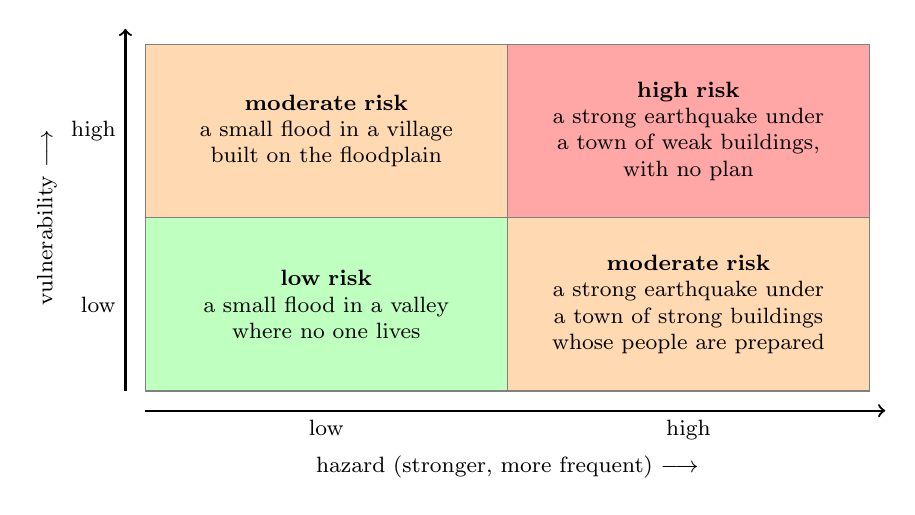
\begin{tikzpicture}[x=1cm, y=1cm, font=\footnotesize,
    cell/.style={minimum width=4.6cm, minimum height=2.2cm, align=center, draw=black!50, text width=4.2cm}]
  \node[cell, fill=green!25] at (2.3,1.1) {\textbf{low risk}\\ a small flood in a valley\\ where no one lives};
  \node[cell, fill=orange!30] at (6.9,1.1) {\textbf{moderate risk}\\ a strong earthquake under\\ a town of strong buildings\\ whose people are prepared};
  \node[cell, fill=orange!30] at (2.3,3.3) {\textbf{moderate risk}\\ a small flood in a village\\ built on the floodplain};
  \node[cell, fill=red!35] at (6.9,3.3) {\textbf{high risk}\\ a strong earthquake under\\ a town of weak buildings,\\ with no plan};
  \draw[->, thick] (0,-0.25) -- (9.4,-0.25);
  \draw[->, thick] (-0.25,0) -- (-0.25,4.6);
  \node[anchor=north] at (4.6,-0.7) {hazard (stronger, more frequent) $\longrightarrow$};
  \node[rotate=90, anchor=south] at (-1.0,2.2) {vulnerability $\longrightarrow$};
  \node[below] at (2.3,-0.25) {low};
  \node[below] at (6.9,-0.25) {high};
  \node[left] at (-0.25,1.1) {low};
  \node[left] at (-0.25,3.3) {high};
\end{tikzpicture}

{\small The \omterm{def:g9:natural-risks:risk}{risk} grid (a sketch). The \omterm{def:g9:natural-risks:risk}{risk} grows with the hazard and
with the \omterm{def:g9:natural-risks:vulnerability}{vulnerability}. Moving a town is rarely possible, and a
hazard cannot be switched off; but its \omterm{def:g9:natural-risks:vulnerability}{vulnerability} can be lowered,
which moves the town down the grid.}
\label{fig:g9:natural-risks:grid}
\end{omfigure}

Armero was a place of high hazard: a snow-capped \omterm{def:g4:volcanoes-earthquakes-first-look:volcano}{volcano} that had woken a
year before, and a town built on the deposits of old mudflows, at the
\omterm{def:g5:water-shapes-the-land:source-mouth}{mouth} of a \omterm{def:g1:landscapes-around-us:landform}{valley} that had carried them before. It was also highly
vulnerable: the scientists lacked instruments and support, the
information given to the authorities was often vague, and no evacuation
plan and no quick way to warn the town existed.
% ledger: usgs:armero

\section{Forecasting and prevention}

Some hazards can be seen coming. A \omterm{def:g5:natural-hazards:storm}{storm} is forecast days ahead
(\cref{ch:g8:fronts-and-weather-maps}); a \omterm{def:g5:water-shapes-the-land:flood}{flood} after heavy \omterm{def:g4:clouds-rain-snow:precipitation}{rain}, hours
to days ahead; a large \omterm{def:g4:volcanoes-earthquakes-first-look:eruption}{eruption} often announces itself days to weeks
ahead, though not always. A \omterm{def:g7:earthquakes:tsunami}{tsunami} crosses an \omterm{def:g2:water-on-earth:ocean}{ocean} in hours, so a
warning can reach distant \omterm{def:g1:landscapes-around-us:water}{coasts} before it does. \omterm{def:g4:volcanoes-earthquakes-first-look:earthquake}{Earthquakes}, on the
other hand, cannot be predicted: scientists can say which \omterm{def:g7:earthquakes:fault}{faults} will
break again one day, never the day.
% ledger: nws:tsunami-speed, usgs:eq-basics, usgs:pinatubo-1991

A forecast, however good, is useful only if something is done before the
hazard strikes. Most of that work is done long before any warning.

\begin{definition}[Prevention]\label{def:g9:natural-risks:prevention}
\emph{Prevention}\index{prevention} is everything done before a \omterm{def:g5:natural-hazards:hazard}{natural
hazard} strikes to lower the \omterm{def:g9:natural-risks:risk}{risk}: knowing where the hazard can strike,
building in safe places and in safe ways, watching the hazard, warning
people and preparing them.
\end{definition}

\omterm{def:g9:natural-risks:prevention}{Prevention} works on both sides of the \omterm{def:g9:natural-risks:risk}{risk} grid. Watching a \omterm{def:g4:volcanoes-earthquakes-first-look:volcano}{volcano} or a
\omterm{def:g1:landscapes-around-us:water}{river} does not make it less dangerous, but it gives time to act. Building
away from the \omterm{def:g5:water-shapes-the-land:flood}{floodplain}, building strong houses, planning the routes to
higher ground and practising them all lower the \omterm{def:g9:natural-risks:vulnerability}{vulnerability}.

\begin{omfigure}
\begin{minipage}[c]{0.44\linewidth}\centering
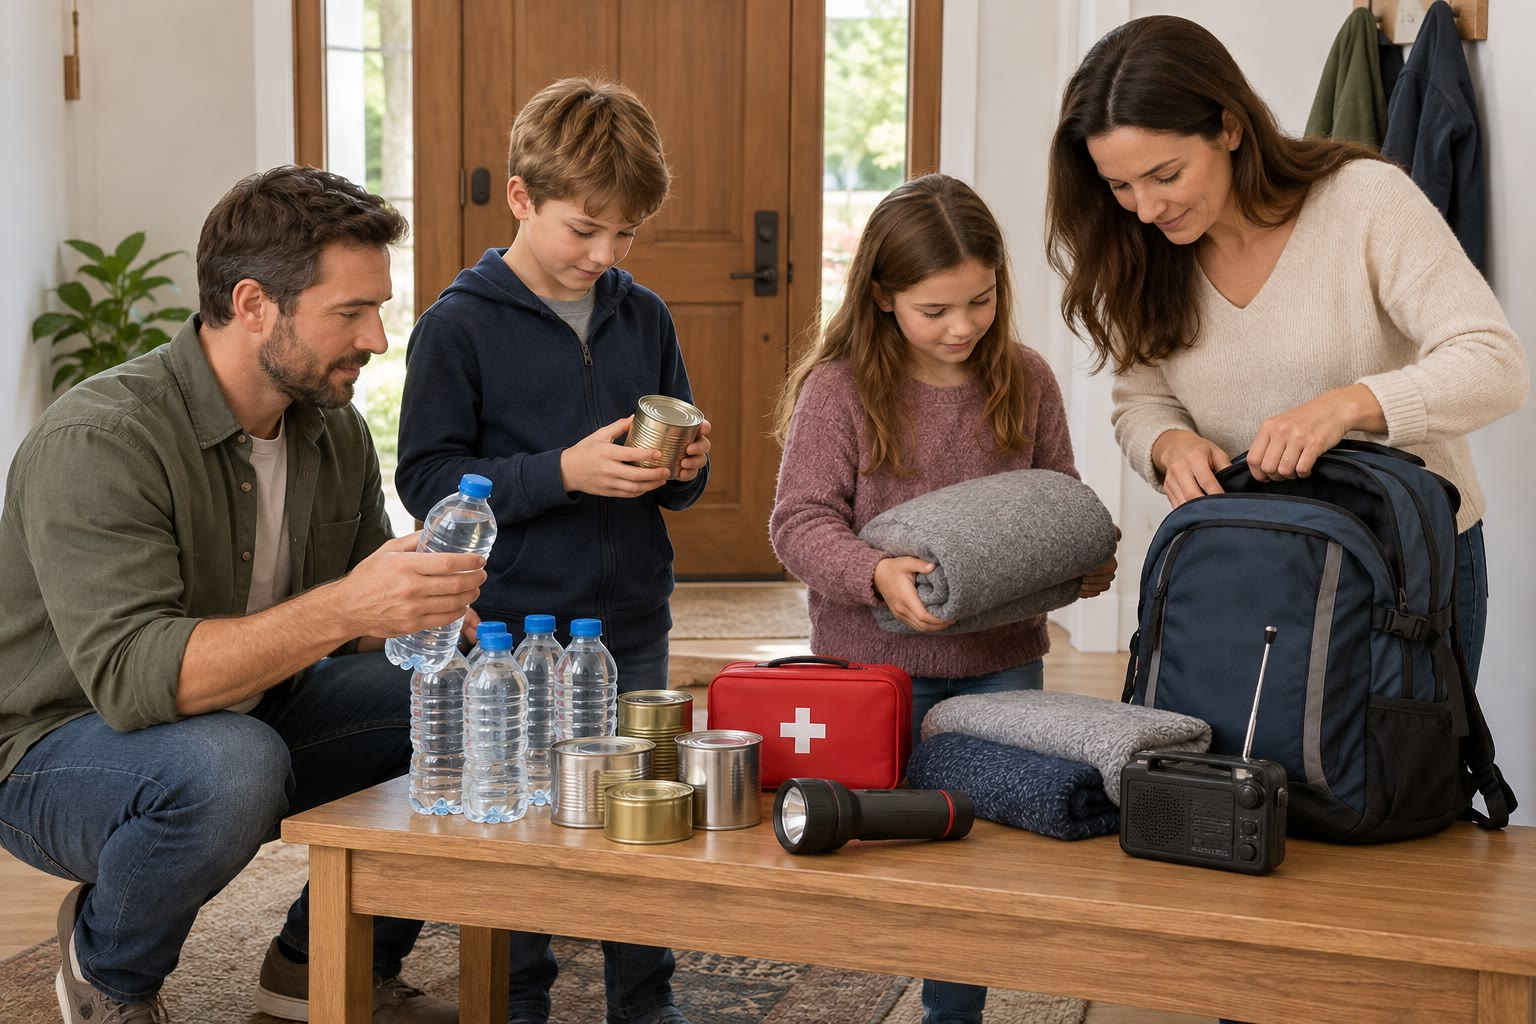
\includegraphics[width=\linewidth]{images/book1/ai/g9-emergency-kit.jpg}
\end{minipage}\hfill
\begin{minipage}[c]{0.52\linewidth}\raggedright
{\small Being prepared: a family checks its emergency kit, kept near
the door, ready to take if they have to leave quickly: water and food
that keeps for several days, a torch, a radio that works without mains
electricity, spare batteries, a first-aid kit and warm blankets
(AI-generated illustration of a generic scene).}
\end{minipage}
% ledger: ready:kit
\label{fig:g9:natural-risks:kit}
\end{omfigure}

\section{Watching volcanoes and faults}

A \omterm{def:g4:volcanoes-earthquakes-first-look:volcano}{volcano} observatory watches the warning signs of \cref{ch:g7:volcanoes}
with instruments that run day and night and send their readings to the
observatory.
% ledger: usgs:hvo-toolkit

\begin{omfigure}
\begin{tikzpicture}[x=1cm, y=1cm, font=\footnotesize, >={Stealth[length=2mm]}]
  % ground and cone
  \fill[black!13] (0,0) -- (0,1.0) -- (3.0,1.2) -- (5.4,3.6) -- (6.4,3.6) -- (8.8,1.2) -- (12,1.0) -- (12,0) -- cycle;
  \draw[black!60] (0,1.0) -- (3.0,1.2) -- (5.4,3.6) -- (6.4,3.6) -- (8.8,1.2) -- (12,1.0);
  % magma chamber and conduit
  \fill[omWarm!70] (5.9,0.6) ellipse (1.5 and 0.38);
  \fill[omWarm!70] (5.75,0.9) rectangle (6.05,3.6);
  \node[white, font=\scriptsize\bfseries] at (5.9,0.58) {magma};
  % gas plume, drifting west
  \fill[black!10] (5.8,3.95) circle (0.3) (5.35,4.35) circle (0.4) (4.75,4.75) circle (0.45);
  % swollen east flank, dashed
  \draw[dashed, omWarm, line width=0.8pt] (6.45,3.7) .. controls (7.5,3.55) and (8.6,2.6) .. (8.85,1.25);
  \draw[->, omWarm] (7.3,2.75) -- (7.7,3.15);
  \node[anchor=west, align=left, text=omWarm!80!black] at (8.2,3.75) {rising magma\\ swells the slope};
  % tiltmeter on the east flank
  \fill[black] (7.75,2.12) rectangle (8.05,2.24);
  \draw[black!70] (8.1,2.2) -- (8.5,2.45);
  \node[anchor=west, align=left] at (8.5,2.55) {tiltmeter: the slope\\ tilts as it swells};
  % GPS receiver on the west flank, and its satellite
  \draw[black, line width=0.6pt] (4.4,2.6) -- (4.4,2.95);
  \fill[black] (4.25,2.95) rectangle (4.55,3.05);
  \draw[black] (4.4,3.05) circle (0.1);
  \draw[black, fill=white] (1.7,4.85) rectangle (2.0,5.05);
  \draw[black] (1.4,4.95) -- (2.3,4.95);
  \node[anchor=east] at (1.35,4.95) {satellite};
  \draw[black!50, dashed] (4.3,3.15) -- (2.05,4.8);
  \draw[black!70] (3.05,2.65) -- (4.2,2.85);
  \node[anchor=east, align=right] at (3.0,2.6) {GPS receiver: the\\ ground moves by\\ millimetres};
  % gas instrument on the crater rim
  \fill[black] (6.45,3.6) rectangle (6.75,3.75);
  \draw[black!70] (6.8,3.75) -- (7.1,4.45);
  \node[anchor=west, align=left] at (7.1,4.6) {gas instrument: the gases\\ escaping from the crater};
  % seismometer (in the ground)
  \fill[black] (2.1,0.95) rectangle (2.4,1.1);
  \node[anchor=north, align=center] at (1.6,0.85) {seismometer:\\ small earthquakes};
  % camera, east, looking at the summit
  \fill[black] (10.7,1.12) rectangle (11.0,1.32);
  \fill[black] (10.7,1.17) -- (10.55,1.12) -- (10.55,1.32) -- (10.7,1.27) -- cycle;
  \node[anchor=north, align=center] at (10.8,0.85) {camera:\\ watches the summit};
\end{tikzpicture}

{\small Watching a \omterm{def:g4:volcanoes-earthquakes-first-look:volcano}{volcano} (a sketch, not to scale). \omterm{def:g7:earthquakes:seismometer}{Seismometers} count
the small \omterm{def:g4:volcanoes-earthquakes-first-look:earthquake}{earthquakes}; tiltmeters and GPS receivers, fixed to the \omterm{def:g3:stones-pebbles-sand:rock}{rock},
measure how the ground tilts and moves as \omterm{def:g7:volcanoes:magma}{magma} gathers below;
other instruments measure the gases that escape; cameras watch the
summit. \omterm{def:g4:clouds-rain-snow:rain-gauge}{Rain gauges} help to tell the signals of the \omterm{def:g4:volcanoes-earthquakes-first-look:volcano}{volcano} from the
effects of heavy \omterm{def:g4:clouds-rain-snow:precipitation}{rain}.}
% ledger: usgs:hvo-toolkit
\label{fig:g9:natural-risks:monitoring}
\end{omfigure}

None of these signs gives the day and the hour of an \omterm{def:g4:volcanoes-earthquakes-first-look:eruption}{eruption}. The
scientists read them together, as a doctor reads several measurements
of a patient, and say how the danger changes; the authorities decide
when to close an area and when to move people out. At Pinatubo this
chain worked. At Nevado del Ruiz, the \omterm{def:g4:volcanoes-earthquakes-first-look:volcano}{volcano} had given signs for a year,
with swarms of \omterm{def:g4:volcanoes-earthquakes-first-look:earthquake}{earthquakes}, but the instruments were few, and the chain
from the scientists to the people of Armero was broken.
% ledger: usgs:armero, usgs:hvo-toolkit, usgs:pinatubo-1991

\omterm{def:g7:earthquakes:fault}{Faults} are watched in the same way, by networks of \omterm{def:g7:earthquakes:seismometer}{seismometers} and of
GPS stations that measure, millimetre by millimetre, how the two sides of
a \omterm{def:g7:earthquakes:fault}{fault} slowly move. This tells which \omterm{def:g7:earthquakes:fault}{faults} are storing up the strain
of the next large \omterm{def:g4:volcanoes-earthquakes-first-look:earthquake}{earthquake}, but not when it will come. For
\omterm{def:g4:volcanoes-earthquakes-first-look:earthquake}{earthquakes}, \omterm{def:g9:natural-risks:prevention}{prevention} is the main defence.
% ledger: usgs:gps, usgs:eq-basics

\section{Hazard maps and flood zones}

The first step of \omterm{def:g9:natural-risks:prevention}{prevention} is to know where a hazard can strike.

\begin{definition}[Hazard map]\label{def:g9:natural-risks:hazard-map}
A \emph{hazard map}\index{hazard map} shows the places that a \omterm{def:g5:natural-hazards:hazard}{natural
hazard} can reach, often with several levels of danger. It is drawn from
what the hazard has done in the past and from the shape of the ground.
\end{definition}

The \omterm{def:g2:drawing-to-map:map}{map} of Nevado del Ruiz, at the start of this chapter, is a
\omterm{def:g9:natural-risks:hazard-map}{hazard map}: the mudflows of the past had followed the \omterm{def:g1:landscapes-around-us:landform}{valleys}, and the
next ones would follow them too. \omterm{def:g5:water-shapes-the-land:flood}{Flood} \omterm{def:g2:drawing-to-map:map}{maps} follow the same idea. Water
spreads over the low, flat ground beside a \omterm{def:g1:landscapes-around-us:water}{river}: the higher the \omterm{def:g5:water-shapes-the-land:flood}{flood},
the wider the band of ground it covers. A \omterm{def:g5:water-shapes-the-land:flood}{flood} \omterm{def:g2:drawing-to-map:map}{map} draws the edge of the
water for a chosen \omterm{def:g5:water-shapes-the-land:flood}{flood}, often the \omterm{def:g5:water-shapes-the-land:flood}{flood} that has a chance of 1 in 100
of being reached or passed in any year. It is called the
\emph{100-year \omterm{def:g5:water-shapes-the-land:flood}{flood}}, but it is not a \omterm{def:g5:water-shapes-the-land:flood}{flood} that comes once a century:
it can come two years in a row.
% ledger: fema:flood-zones

\begin{omfigure}
\begin{tikzpicture}
\begin{axis}[axis equal image, xmin=3.5, xmax=7, ymin=2.7, ymax=5.5, width=11.5cm,
  enlargelimits=false, tick label style={font=\scriptsize}, xlabel={east (km)},
  ylabel={north (km)}, label style={font=\small}, xtick={3.5,4,...,7}, ytick={3,3.5,...,5.5},
  clip mode=individual]
\addplot[contour] table {figdata/out/grade-9-flood_zone-contours.dat};
\addplot[index contour] table {figdata/out/grade-9-flood_zone-index.dat};
\addplot[fill=omSea, draw=blue!40, line width=0.3pt] table {figdata/out/grade-9-flood_zone-zone10.dat} -- cycle;
\addplot[fill=blue!25, draw=blue!50, line width=0.3pt] table {figdata/out/grade-9-flood_zone-zone.dat} -- cycle;
\addplot[fill=blue!50, draw=none] table {figdata/out/grade-9-flood_zone-zone2.dat} -- cycle;
\addplot[only marks, mark=none, point meta=explicit symbolic, nodes near coords,
  nodes near coords align={center}, nodes near coords style={font=\tiny, fill=white, inner sep=0.6pt, text=omContour}]
  table[meta=z] {figdata/out/grade-9-flood_zone-index-lab.dat};
\addplot[river] table {figdata/out/grade-9-flood_zone-river.dat};
\end{axis}
\end{tikzpicture}

\smallskip
\begin{tikzpicture}[font=\footnotesize]
  \node[anchor=east] at (0,0.125) {flood above the river:};
  \fill[blue!50] (0.2,0) rectangle (0.7,0.25); \node[anchor=west] at (0.8,0.125) {\qty{2}{m}};
  \fill[blue!25, draw=blue!50, line width=0.3pt] (1.9,0) rectangle (2.4,0.25); \node[anchor=west] at (2.5,0.125) {\qty{5}{m}};
  \fill[omSea, draw=blue!40, line width=0.3pt] (3.6,0) rectangle (4.1,0.25); \node[anchor=west] at (4.2,0.125) {\qty{10}{m}};
\end{tikzpicture}

{\small The \omterm{def:g5:water-shapes-the-land:flood}{floodplain} of the \omterm{def:g1:landscapes-around-us:water}{river} of the Varden Hills, which flows east.
Each shade is the ground that a \omterm{def:g5:water-shapes-the-land:flood}{flood} would cover if it rose 2, 5 or
\qty{10}{m} above the normal level of the \omterm{def:g1:landscapes-around-us:water}{river}: each zone contains the
smaller ones. The zones stay narrow because the sides of the \omterm{def:g1:landscapes-around-us:landform}{valley} rise
quickly from its flat floor. The thin lines join points at the same
height, every \qty{10}{m}, labelled every \qty{50}{m}; such \omterm{def:g2:drawing-to-map:map}{maps} are the
subject of \cref{ch:g9:maps-of-the-earth}.}
% ledger: (invented region: figdata/grade-9/flood_zone.py, parts zone2, zone, zone10)
\label{fig:g9:natural-risks:flood-zones}
\end{omfigure}

\begin{method}[Reading a flood-zone map]
\begin{enumerate}
  \item Find which \omterm{def:g5:water-shapes-the-land:flood}{flood} the zone stands for: how high above the \omterm{def:g1:landscapes-around-us:water}{river},
        or how often it may come.
  \item Locate the place on the \omterm{def:g2:drawing-to-map:map}{map}, with the \omterm{def:g2:drawing-to-map:scale}{scale} bar or the grid.
  \item If the place lies inside the shaded zone, that \omterm{def:g5:water-shapes-the-land:flood}{flood} would reach
        it; if it lies outside, it would stay dry in that \omterm{def:g5:water-shapes-the-land:flood}{flood}, not in
        every \omterm{def:g5:water-shapes-the-land:flood}{flood}.
  \item To compare places, use their heights above the \omterm{def:g1:landscapes-around-us:water}{river}: the
        lower, the more often flooded.
\end{enumerate}
\end{method}

\begin{example}[Three houses beside the river]
On a \omterm{def:g2:drawing-to-map:map}{map} like the one above, a house stands on
ground \qty{3}{m} above the \omterm{def:g1:landscapes-around-us:water}{river}. A \omterm{def:g5:water-shapes-the-land:flood}{flood} \qty{2}{m} above the \omterm{def:g1:landscapes-around-us:water}{river}
does not reach it; \omterm{def:g5:water-shapes-the-land:flood}{floods} of 5 and \qty{10}{m} do. A second house,
\qty{8}{m} above the \omterm{def:g1:landscapes-around-us:water}{river}, is reached only by the \qty{10}{m} \omterm{def:g5:water-shapes-the-land:flood}{flood}, and
a third, on a slope \qty{30}{m} above the \omterm{def:g1:landscapes-around-us:water}{river}, by none of the three.
The first house is the most vulnerable: smaller \omterm{def:g5:water-shapes-the-land:flood}{floods}, which come more
often, are enough to reach it.
\end{example}

\section{Building to resist earthquakes}

In an \omterm{def:g4:volcanoes-earthquakes-first-look:earthquake}{earthquake}, the ground moves back and forth under a building, and
the building is shaken from below; in a strong \omterm{def:g4:volcanoes-earthquakes-first-look:earthquake}{earthquake}, the danger
comes above all from buildings that crack and fall. Engineers cannot stop
the shaking, but they can build so that the structure carries the forces
of the shaking without falling.
% ledger: iris:better-wall

\begin{omfigure}
\begin{tikzpicture}[x=1cm, y=1cm, font=\footnotesize, >={Stealth[length=2mm]}]
  % panel 1: a frame that leans
  \begin{scope}
    \fill[black!13] (-0.3,-0.25) rectangle (3.0,0);
    \draw[black!35, dashed] (0.2,0) rectangle (2.5,2.6);
    \draw[black, line width=1.2pt] (0.2,0) -- (0.75,2.6) -- (3.05,2.6) -- (2.5,0);
    \draw[black, line width=1.2pt] (0.47,1.3) -- (2.77,1.3);
    \draw[<->] (0.2,-0.45) -- (1.0,-0.45);
    \node[align=center, anchor=north] at (1.35,-0.65) {(a) a bare frame\\ leans and can fall};
  \end{scope}
  % panel 2: braces
  \begin{scope}[xshift=3.7cm]
    \fill[black!13] (-0.3,-0.25) rectangle (3.0,0);
    \draw[black, line width=1.2pt] (0.2,0) rectangle (2.5,2.6);
    \draw[black, line width=1.2pt] (0.2,1.3) -- (2.5,1.3);
    \draw[omWarm, line width=1pt] (0.2,0) -- (2.5,1.3) (2.5,0) -- (0.2,1.3)
                                  (0.2,1.3) -- (2.5,2.6) (2.5,1.3) -- (0.2,2.6);
    \node[align=center, anchor=north] at (1.35,-0.65) {(b) diagonal braces\\ keep its shape};
  \end{scope}
  % panel 3: shear wall
  \begin{scope}[xshift=7.4cm]
    \fill[black!13] (-0.3,-0.25) rectangle (3.0,0);
    \draw[black, line width=1.2pt] (0.2,0) rectangle (2.5,2.6);
    \draw[black, line width=1.2pt] (0.2,1.3) -- (2.5,1.3);
    \fill[omWarm!35] (1.6,0) rectangle (2.5,2.6);
    \draw[black, line width=0.6pt] (1.6,0) rectangle (2.5,2.6);
    \node[align=center, anchor=north] at (1.35,-0.65) {(c) a stiff shear wall\\ from top to bottom};
  \end{scope}
  % panel 4: base isolation
  \begin{scope}[xshift=11.1cm]
    \fill[black!13] (-0.3,-0.25) rectangle (3.0,0);
    \foreach \x in {0.35,1.35,2.35} \fill[omSea, draw=black!60, rounded corners=1pt] (\x-0.18,0) rectangle (\x+0.18,0.3);
    \draw[black, line width=1.2pt] (0.15,0.3) -- (2.55,0.3);
    \draw[black, line width=1.2pt] (0.2,0.3) rectangle (2.5,2.7);
    \draw[black, line width=1.2pt] (0.2,1.5) -- (2.5,1.5);
    \draw[<->] (0.2,-0.45) -- (1.0,-0.45);
    \node[align=center, anchor=north] at (1.35,-0.65) {(d) isolators let the\\ ground move beneath};
  \end{scope}
\end{tikzpicture}

{\small Four frames shaken by the same ground (a sketch). A frame of
posts and beams alone leans over and can collapse (a). Diagonal braces
(b) and stiff shear walls (c) stop it from leaning; strong joints between
the beams and the posts hold it together. Isolators placed
under the building (d) give way as the ground moves, so that much less of
the motion reaches the building.}
% ledger: iris:better-wall, explo:base-isolation
\label{fig:g9:natural-risks:buildings}
\end{omfigure}

The same principles serve a house, a school or a bridge. They are
easiest to apply when the building is designed, rather than added to an
old building afterwards.

\begin{inthelab}[A tower on a shaking tray]
Indoors, build two small towers of the same height from drinking straws
or wooden sticks and modelling clay, as two-storey frames. Give the second
one diagonal braces on every side. Stand both on a tray, then slide the
tray quickly back and forth, gently at first, then harder. Which tower
leans first? Which one keeps its shape? Then put the bare tower on four
marbles under a light card, and shake again: what changes?
\end{inthelab}

\section{Warnings in time}

The last part of \omterm{def:g9:natural-risks:prevention}{prevention} is the warning. For \omterm{def:g7:earthquakes:tsunami}{tsunamis}, it starts on
the floor of the \omterm{def:g2:water-on-earth:ocean}{ocean}. At sites near where destructive \omterm{def:g7:earthquakes:tsunami}{tsunamis} have
started before, a pressure recorder lies on the \omterm{def:g2:water-on-earth:ocean}{sea} floor and reads the
weight of the water above it every \qty{15}{s}, which gives the height
of the \omterm{def:g2:water-on-earth:ocean}{sea} surface. It sends its readings by sound through the water to a
buoy moored at the surface, and the buoy relays them by satellite to the
\omterm{def:g7:earthquakes:tsunami}{tsunami} warning centres. A rise of the \omterm{def:g2:water-on-earth:ocean}{sea} far from any \omterm{def:g1:landscapes-around-us:water}{coast} shows a
\omterm{def:g7:earthquakes:tsunami}{tsunami} on its way, hours before it reaches distant shores.
% ledger: ndbc:dart, nws:tsunami-speed

\begin{omfigure}
\begin{minipage}[c]{0.4\linewidth}\centering
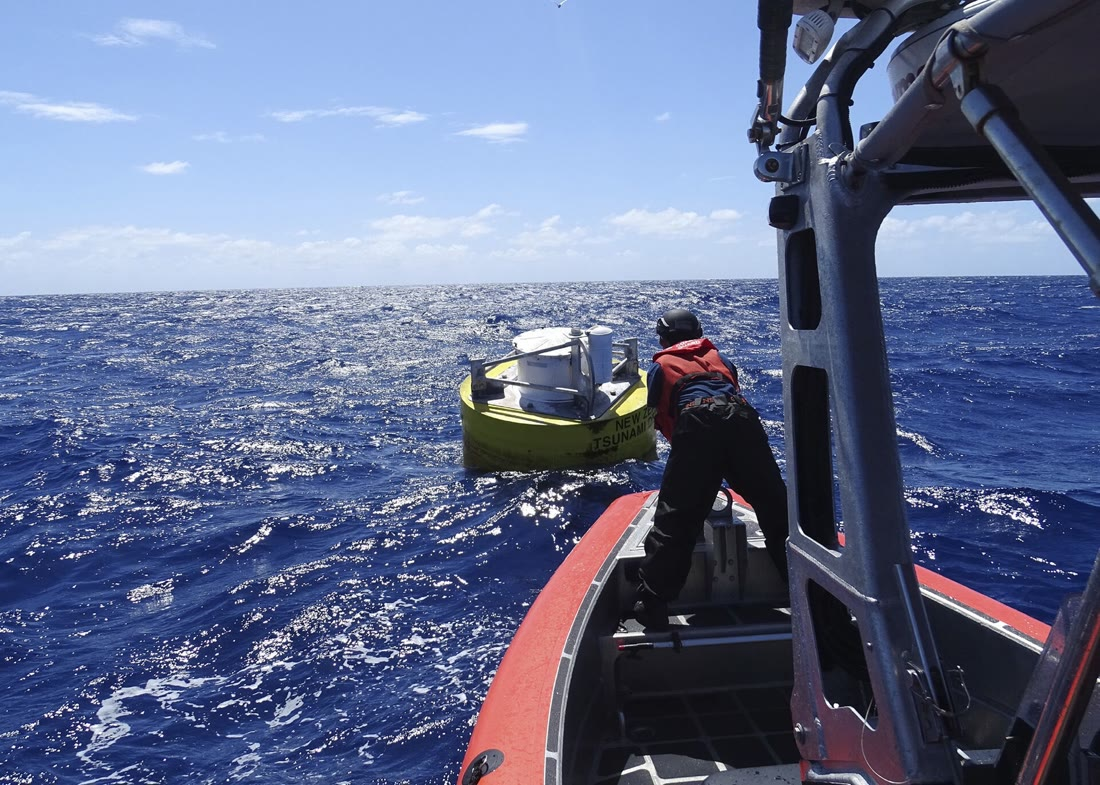
\includegraphics[width=\linewidth]{images/book1/g9-dart-buoy.jpg}
\end{minipage}\hfill
\begin{minipage}[c]{0.56\linewidth}\raggedright
{\small A crew member of a United States Coast Guard ship inspects a
\omterm{def:g7:earthquakes:tsunami}{tsunami} warning buoy in the Pacific \omterm{def:g2:water-on-earth:ocean}{Ocean}, in November 2021. The buoy
floats above a pressure recorder on the \omterm{def:g2:water-on-earth:ocean}{sea} floor, thousands of metres
below. U.S. Coast Guard (public domain, via Wikimedia Commons).}
\end{minipage}
% ledger: commons:dart-buoy
\label{fig:g9:natural-risks:buoy}
\end{omfigure}

\begin{history}[A network of buoys]
In 2001 the first array of six such stations was complete, in the
Pacific \omterm{def:g2:water-on-earth:ocean}{Ocean}. After the \omterm{def:g7:earthquakes:tsunami}{tsunami} of December 2004, which reached the
\omterm{def:g1:landscapes-around-us:water}{coasts} of the Indian \omterm{def:g2:water-on-earth:ocean}{Ocean} with no warning system in place
(\cref{ch:g7:earthquakes}), the network grew: by March 2008, there were
39 stations.
\end{history}
% ledger: ndbc:dart

A warning saves lives only if it reaches people who know what to do with
it: the routes to higher ground are signposted and practised, the
emergency kit is ready, schools hold drills. At Armero, the hazard was
known and the \omterm{def:g2:drawing-to-map:map}{map} was drawn; the warning never reached the town.
% ledger: ready:kit, usgs:armero

\section{Exercises}

\begin{exercise}[$\star$]\label{exo:g9:natural-risks:1}
Hazard or \omterm{def:g9:natural-risks:vulnerability}{vulnerability}? (a) A \omterm{def:g1:landscapes-around-us:water}{river} that \omterm{def:g5:water-shapes-the-land:flood}{floods} almost every spring.
(b) A village with no warning system. (c) Heavy houses of brick with no
frame. (d) A strong \omterm{def:g4:volcanoes-earthquakes-first-look:earthquake}{earthquake} on a nearby \omterm{def:g7:earthquakes:fault}{fault}. (e) A town built at the
\omterm{def:g5:water-shapes-the-land:source-mouth}{mouth} of a \omterm{def:g1:landscapes-around-us:landform}{valley} where mudflows have run before.
\end{exercise}

\begin{exercise}[$\star$]\label{exo:g9:natural-risks:2}
True or false? Correct the false sentences. (a) A \omterm{def:g5:natural-hazards:hazard}{natural hazard} in a
place where no one lives is a high \omterm{def:g9:natural-risks:risk}{risk}. (b) \omterm{def:g9:natural-risks:prevention}{Prevention} can lower the
\omterm{def:g9:natural-risks:vulnerability}{vulnerability} of a town. (c) A \omterm{def:g9:natural-risks:hazard-map}{hazard map} shows where a hazard can strike.
(d) A good warning system makes a \omterm{def:g4:volcanoes-earthquakes-first-look:volcano}{volcano} less dangerous.
\end{exercise}

\begin{exercise}[$\star$]\label{exo:g9:natural-risks:3}
For each hazard, say whether it can be forecast days or hours ahead:
(a) a \omterm{def:g5:natural-hazards:storm}{storm}; (b) a \omterm{def:g5:water-shapes-the-land:flood}{flood} after heavy \omterm{def:g4:clouds-rain-snow:precipitation}{rain}; (c) an \omterm{def:g4:volcanoes-earthquakes-first-look:earthquake}{earthquake}; (d) the
arrival of a \omterm{def:g7:earthquakes:tsunami}{tsunami} on a \omterm{def:g1:landscapes-around-us:water}{coast} far from where it started.
\end{exercise}

\begin{exercise}[$\star$]\label{exo:g9:natural-risks:4}
% ledger: usgs:hvo-toolkit
Use the drawing of a watched \omterm{def:g4:volcanoes-earthquakes-first-look:volcano}{volcano}. What does each instrument measure,
and what warning sign of an \omterm{def:g4:volcanoes-earthquakes-first-look:eruption}{eruption} does it watch for? (a) A \omterm{def:g7:earthquakes:seismometer}{seismometer}.
(b) A tiltmeter. (c) A GPS receiver. (d) A gas instrument.
\end{exercise}

\begin{exercise}[$\star\star$]\label{exo:g9:natural-risks:5}
% ledger: usgs:armero
In 1985, the mudflows of Nevado del Ruiz reached Armero, \qty{45}{km}
away, about two hours after the \omterm{def:g4:volcanoes-earthquakes-first-look:eruption}{eruption}. (a) What was their average
speed, in kilometres per hour? (b) A person walks at about
\qty{4}{km/h}. How far could the people have walked in two hours?
(c) Why did they not leave? (d) Give two things that could have saved
them.
\end{exercise}

\begin{exercise}[$\star\star$]\label{exo:g9:natural-risks:6}
% ledger: (invented region: figdata/grade-9/flood_zone.py)
Use the flood-zone \omterm{def:g2:drawing-to-map:map}{map} of the Varden Hills. (a) Which \omterm{def:g5:water-shapes-the-land:flood}{flood} covers the
widest band? (b) With the grid of the \omterm{def:g2:drawing-to-map:map}{map}, measure the width of each
zone across the \omterm{def:g1:landscapes-around-us:landform}{valley} at \qty{5}{km} east. (c) A barn stands on ground
\qty{6}{m} above the \omterm{def:g1:landscapes-around-us:water}{river}.
Which of the three \omterm{def:g5:water-shapes-the-land:flood}{floods} reach it? (d) Why is the \omterm{def:g5:water-shapes-the-land:flood}{flood} \qty{2}{m} above
the \omterm{def:g1:landscapes-around-us:water}{river} the one that comes most often?
\end{exercise}

\begin{exercise}[$\star\star$]\label{exo:g9:natural-risks:7}
Place each situation on the \omterm{def:g9:natural-risks:risk}{risk} grid (low or high hazard, low or high
\omterm{def:g9:natural-risks:vulnerability}{vulnerability}) and say whether the \omterm{def:g9:natural-risks:risk}{risk} is low, moderate or high.
(a) Strong buildings and drills in a town on an active \omterm{def:g7:earthquakes:fault}{fault}. (b) A
camp site on the \omterm{def:g5:water-shapes-the-land:flood}{floodplain} of a \omterm{def:g1:landscapes-around-us:water}{river} that rarely \omterm{def:g5:water-shapes-the-land:flood}{floods}. (c) A village
of weak houses at the foot of an active \omterm{def:g4:volcanoes-earthquakes-first-look:volcano}{volcano}, with no observatory.
(d) A town on a hilltop far from any \omterm{def:g7:earthquakes:fault}{fault}, \omterm{def:g1:landscapes-around-us:water}{river} or \omterm{def:g4:volcanoes-earthquakes-first-look:volcano}{volcano}.
\end{exercise}

\begin{exercise}[$\star\star$]\label{exo:g9:natural-risks:8}
% ledger: iris:better-wall, explo:base-isolation
Three schools are built on the same ground. School A is a frame of posts
and beams with brick walls between them; school B has the same frame
with diagonal braces and two shear walls; school C has the frame of B,
standing on isolators. (a) Rank them from the safest to the least safe
in an \omterm{def:g4:volcanoes-earthquakes-first-look:earthquake}{earthquake}. (b) Explain what the braces do. (c) Explain what the
isolators do.
\end{exercise}

\begin{exercise}[$\star\star$]\label{exo:g9:natural-risks:9}
% ledger: fema:flood-zones
A \omterm{def:g5:water-shapes-the-land:flood}{flood} \omterm{def:g2:drawing-to-map:map}{map} shows the 100-year \omterm{def:g5:water-shapes-the-land:flood}{flood}, which has a chance of 1 in 100 of
being reached or passed in any year. (a) Write this chance as a
percentage. (b) A neighbour says: ``The 100-year \omterm{def:g5:water-shapes-the-land:flood}{flood} came last year,
so we are safe for 99 years.'' What is wrong? (c) On average, how many
such \omterm{def:g5:water-shapes-the-land:flood}{floods} would come in 300 years?
\end{exercise}

\begin{exercise}[$\star\star$]\label{exo:g9:natural-risks:10}
% ledger: ndbc:dart, nws:tsunami-speed
A \omterm{def:g7:earthquakes:tsunami}{tsunami} warning station reads the \omterm{def:g2:water-on-earth:ocean}{sea} floor pressure every
\qty{15}{s}. (a) How many readings does it make in one hour? (b) In one
year of 365 days? Write the answer in scientific notation. (c) A \omterm{def:g7:earthquakes:tsunami}{tsunami}
crosses the deep \omterm{def:g2:water-on-earth:ocean}{ocean} at about \qty{800}{km/h}. How long does it take to
reach a \omterm{def:g1:landscapes-around-us:water}{coast} \qty{2400}{km} away? (d) Why does that time matter?
\end{exercise}

\begin{exercise}[$\star\star\star$]\label{exo:g9:natural-risks:11}
% ledger: ready:kit
A family of four prepares an emergency kit with water for 3 days, at
about \qty{3.8}{L} per person per day, for drinking and washing.
(a) How many litres of water do they need? (b) How many bottles of
\qty{1.5}{L} is that? (c) Name four other things the kit holds, and
say why each one is useful. (d) Why is the kit kept near the door?
\end{exercise}

\begin{exercise}[$\star\star\star$]\label{exo:g9:natural-risks:12}
% ledger: usgs:armero, usgs:hvo-toolkit
A town lies beside a \omterm{def:g1:landscapes-around-us:water}{river}, at the \omterm{def:g5:water-shapes-the-land:source-mouth}{mouth} of a \omterm{def:g1:landscapes-around-us:landform}{valley} that comes down
from a snow-capped \omterm{def:g4:volcanoes-earthquakes-first-look:volcano}{volcano}. Old mudflow deposits lie under its streets.
The \omterm{def:g4:volcanoes-earthquakes-first-look:volcano}{volcano} has begun to shake with small \omterm{def:g4:volcanoes-earthquakes-first-look:earthquake}{earthquakes}. Write a
prevention plan of five points for the town. For each point, say
whether it acts on the hazard side (knowing and watching the hazard) or
on the \omterm{def:g9:natural-risks:vulnerability}{vulnerability} side of the \omterm{def:g9:natural-risks:risk}{risk}.
\end{exercise}

\section{Problem: Where should the new school go?}

\begin{problem}[{Weekend problem --- a new school is placed on the map of
the Varden Hills, away from floods, steep slopes and the fault; the final
answer is the number of houses inside the flood zone}]
\label{pb:g9:natural-risks:1}
% ledger: (invented region: figdata/grade-9/flood_zone.py: sites A, B, C; 17 of 28 houses in the 5 m zone)
The village of the Varden Hills needs a new school, and three sites are
offered: A, B and C, on the \omterm{def:g2:drawing-to-map:map}{map} below. The \omterm{def:g5:water-shapes-the-land:flood}{flood} zone shaded on the \omterm{def:g2:drawing-to-map:map}{map} is
all the ground less than \qty{5}{m} above the \omterm{def:g1:landscapes-around-us:water}{river}, which a large \omterm{def:g5:water-shapes-the-land:flood}{flood}
would cover. The table gives, for each site, the elevation of the
ground, the level of the \omterm{def:g1:landscapes-around-us:water}{river} beside it, and how much the ground rises
over \qty{200}{m} measured flat across the slope.

\begin{center}
{\small
\begin{tabular}{|c|c|c|c|}
\hline
site & ground elevation & \omterm{def:g1:landscapes-around-us:water}{river} level beside it & rise of the ground over \qty{200}{m} \\
\hline
A & \qty{137}{m} & \qty{137}{m} & \qty{1.4}{m} \\
B & \qty{276}{m} & \qty{126}{m} & \qty{83}{m} \\
C & \qty{236}{m} & \qty{143}{m} & \qty{20}{m} \\
\hline
\end{tabular}}
\end{center}

\begin{omfigure}
\begin{tikzpicture}
\begin{axis}[axis equal image, xmin=3.5, xmax=7, ymin=2.7, ymax=5.5, width=11.5cm,
  enlargelimits=false, tick label style={font=\scriptsize}, xlabel={east (km)},
  ylabel={north (km)}, label style={font=\small}, xtick={3.5,4,...,7}, ytick={3,3.5,...,5.5}]
\addplot[contour] table {figdata/out/grade-9-flood_zone-contours.dat};
\addplot[index contour] table {figdata/out/grade-9-flood_zone-index.dat};
\addplot[fill=blue!25, draw=blue!50, line width=0.3pt] table {figdata/out/grade-9-flood_zone-zone.dat} -- cycle;
\addplot[only marks, mark=none, point meta=explicit symbolic, nodes near coords,
  nodes near coords align={center}, nodes near coords style={font=\tiny, fill=white, inner sep=0.6pt, text=omContour}]
  table[meta=z] {figdata/out/grade-9-flood_zone-index-lab.dat};
\addplot[river] table {figdata/out/grade-9-flood_zone-river.dat};
\addplot[fault] table {figdata/out/shared-region-fault.dat};
\addplot[only marks, mark=square*, mark size=1.5pt, mark options={fill=black}] table {figdata/out/grade-9-flood_zone-houses-in.dat};
\addplot[only marks, mark=square*, mark size=1.5pt, mark options={fill=black}] table {figdata/out/grade-9-flood_zone-houses-out.dat};
\addplot[only marks, mark=*, mark size=2.6pt, mark options={fill=omWarm, draw=black}, point meta=explicit symbolic,
  nodes near coords, nodes near coords align={anchor=south west},
  nodes near coords style={font=\small\bfseries, fill=white, inner sep=1pt, xshift=2.5pt, yshift=2.5pt}]
  table[meta=name] {figdata/out/grade-9-flood_zone-sites.dat};
\node[font=\footnotesize, fill=white, inner sep=1pt, anchor=west] at (axis cs:6.42,5.05) {fault};
\coordinate (na) at (axis cs:3.7,4.75);
\fill[black] (axis cs:5.8,2.85) rectangle (axis cs:5.925,2.9);
\fill[white] (axis cs:5.925,2.85) rectangle (axis cs:6.05,2.9);
\fill[black] (axis cs:6.05,2.85) rectangle (axis cs:6.175,2.9);
\fill[white] (axis cs:6.175,2.85) rectangle (axis cs:6.3,2.9);
\draw[black, line width=0.4pt] (axis cs:5.8,2.85) rectangle (axis cs:6.3,2.9);
\node[font=\footnotesize, above, inner sep=1.5pt, fill=white] at (axis cs:6.05,2.9) {\qty{500}{m}};
\end{axis}
\fill[white, opacity=0.85] ($(na)+(-0.35,-0.1)$) rectangle ($(na)+(0.35,1.45)$);
\pic at (na) {northarrow};
\end{tikzpicture}

{\small The village, the three school sites and the \omterm{def:g5:water-shapes-the-land:flood}{flood} zone (shaded),
on the \omterm{def:g2:drawing-to-map:map}{map} of the Varden Hills (thin lines of equal height every
\qty{10}{m}). Each small black square is a house. The thick black line
is a \omterm{def:g7:earthquakes:fault}{fault}.}
\label{fig:g9:natural-risks:school-map}
\end{omfigure}

\noindent\textbf{Part I --- The flood zone.}\par\nopagebreak
\begin{enumerate}[beginpenalty=10000]
  \item Using the \omterm{def:g1:landscapes-around-us:water}{river} levels of the table, say which way the \omterm{def:g1:landscapes-around-us:water}{river}
        flows.
  \item Compute the height of each site above the \omterm{def:g1:landscapes-around-us:water}{river} beside it.
  \item Which of the three sites lies in the \omterm{def:g5:water-shapes-the-land:flood}{flood} zone?
  \item Use the \omterm{def:g2:drawing-to-map:scale}{scale} bar to measure the width of the \omterm{def:g5:water-shapes-the-land:flood}{flood} zone, across
        the \omterm{def:g1:landscapes-around-us:landform}{valley}, at site A.
\end{enumerate}

\noindent\textbf{Part II --- The slopes and the fault.}\par\nopagebreak
\begin{enumerate}[resume, beginpenalty=10000]
  \item A slope in percent is the rise of the ground for every
        \qty{100}{m} measured flat. Compute the slope at each site.
  \item Which site would be exposed to a \omterm{def:g5:natural-hazards:landslide}{landslide}? Explain.
  \item Use the \omterm{def:g2:drawing-to-map:scale}{scale} bar to estimate the distance from each site to the
        \omterm{def:g7:earthquakes:fault}{fault}.
  \item Suppose that the \omterm{def:g7:earthquakes:fault}{fault} could still move. Why is the ground right
        on top of it a bad place for a school?
\end{enumerate}

\noindent\textbf{Part III --- Choosing.}\par\nopagebreak
\begin{enumerate}[resume, beginpenalty=10000]
  \item Draw a table with one row per site and three columns: in the
        \omterm{def:g5:water-shapes-the-land:flood}{flood} zone? steep slope? on the \omterm{def:g7:earthquakes:fault}{fault}? Fill it with yes or no.
  \item Which site would you choose? Justify your choice with the table.
  \item The chosen site still lies in a region where the ground can
        shake. Name two ways of building the school, and one habit of its
        pupils, that lower its \omterm{def:g9:natural-risks:vulnerability}{vulnerability}.
  \item The school will also serve as a shelter during \omterm{def:g5:water-shapes-the-land:flood}{floods}. Count the
        houses of the village that stand inside the \omterm{def:g5:water-shapes-the-land:flood}{flood} zone. What
        fraction of all the houses is that?
\end{enumerate}
\end{problem}
